Having introduced the matrix groups, we'll next discuss some important subgroups of $GL(n,\RR)$. First, the \term{orthogonal groups.}
\begin{defn}
Orthogonal groups $O(n)$ are the matrix groups which preserve the Euclidean inner product,
\begin{equation}
O(n)=\set{M\in GL(n,\RR): M^T M = I_N}.
\end{equation}
Their elements correspond to orthogonal transformations, so that for $\vec{v}\in \RR^n$, an orthogonal matrix $M$ acts on $\vec{v}$ by matrix multiplication,
$$\vec{v}'=M\cdot \vec{v}$$
and so in particular
$$|\vec{v}'|^2={\vec{v}'}^T \cdot \vec{v}' = \vec{v}^T \cdot M^T M \cdot \vec{v}= \vec{v}^T \cdot \vec{v}=|\vec{v}|^2.$$
It also follows that $\forall M\in O(n), \det(M^TM)=\det(M)^2 = \det(I_n) = 1 \implies \det M =\pm 1$.
\end{defn}
$\det M$ is a smooth function of the coordinates, but our constraint equation means that $\det M$ can only take on one of two discrete values. The orthogonal group $O(n)$ has therefore two connected components corresponding to $\det M = +1$ and $\det M = -1$. The connected component containing the origin ($\det M = +1$) is the special orthogonal group $SO(n)$.
\begin{defn}
The \term{special orthogonal groups} $SO(n)$ are the subset of orthogonal groups which also preserve orientation (i.e. no reflections):
$$SO(n)\equiv \set{M\in O(n): \det M = +1}.$$
That is, elements of $SO(n)$ preserve the sign of the volume element in $\RR^n$,
$$\Omega= \epsilon^{i_1 i_2 \ldots i_n} v_1^{i_1}v_2^{i_2}\ldots v_n^{i_n}.$$
\end{defn}
In contrast, $O(n)$ matrices may include reflections as well as rotations when $\det M = -1$.

\begin{ex}\label{groupaxiomsson}
Check the group axioms for $SO(n)$.\footnote{As usual, we need to check closure and inverses. The identity matrix $I$ satisfies $I^TI=I$ and $\det I=1$, and associativity follows from standard matrix multiplication. Inverses: if $M\in SO(n)$, then $M^{-1}$ is defined by $MM^{-1}=I$. But $\det(MM^{-1})=\det(M)\det(M^{-1})=(1)\det(M^{-1})=\det I = 1$, so $\det(M^{-1})=1$. We also check that the inverse of an orthogonal matrix is also orthogonal: $M M^{-1}=I$, so $(M^{-1})^T (M^T)= (M^{-1})^T M^{-1} =I^T = I$. Closure: $\forall M,N \in SO(n), \det(MN)=\det(M)\det(N)=(1)(1)=1$ and $(MN)^T(MN)=N^TM^T M N= I$, so $MN\in SO(n)$. \qed}
Show that $\dim(O(n))=\dim(SO(n))=\frac{1}{2} n(n-1)$.\footnote{This can be seen by writing a matrix $M\in SO(n)$ as a row of $n$ column vectors $(\vec{x_1},\vec{x_2},\ldots,\vec{x_n})$. Then the condition that $M^T M = 1$ is equivalent to
$\begin{pmatrix}
\vec{x_1}\cdot \vec{x_1} & \vec{x_1}\cdot \vec{x_2} & \ldots &\vec{x_1}\cdot \vec{x_n}\\
\vec{x_2}\cdot \vec{x_1} & \vec{x_2}\cdot \vec{x_2} & \ldots &\vec{x_2}\cdot \vec{x_n}\\
\vdots\\
\vec{x_n}\cdot \vec{x_1}& \ldots & \ldots & \vec{x_n} \cdot \vec{x_n}
\end{pmatrix}= I_n.$
We see that by the symmetry of the explicit form of $M^T M$, we get $1+2+3+\ldots+n = n(n+1)/2$ independent constraints on the $n^2$ entries of $M$. Applying our theorem, we find that the resulting manifold has dimension $n^2-n(n+1)/2=n(n-1)/2$.
} 
\end{ex}

Orthogonal matrices have some nice properties. Let $M \in O(n)$ be an orthogonal matrix and suppose that $\vec{v}_\lambda$ is an eigenvector of $M$ with eigenvalue $\lambda.$ Then the following is true:
\begin{enumerate}
\item If $\lambda$ is an eigenvalue, then $\lambda^*$ is also an eigenvalue (eigenvalues of $M$ come in complex conjugate pairs).
\item $|\lambda|^2=1$.
\end{enumerate}
The proof is as follows:
\begin{enumerate}
\item $M\cdot \vec{v}_\lambda = \lambda \vec{v}_\lambda \implies M\cdot \vec{v}_\lambda^* = \lambda^* \vec{v}_\lambda^*$ (since $M$ is a real matrix).\footnote{This is generally true of real matrices with complex eigenvalues-- it's not specific to orthogonal matrices.}
\item For any complex vector $\vec{v}$, we have
$$(M\cdot \vec{v}^*)^T \cdot M \cdot \vec{v} = \vec{v}^\dagger \cdot M^T M \cdot \vec{v} = \vec{v}^\dagger \cdot \vec{v}.$$ Now if $\vec{v}=\vec{v}_\lambda$, then
$$(M\cdot \vec{v}_\lambda^*)^T \cdot M \cdot \vec{v}_\lambda=(\lambda^* \vec{v}^*_\lambda)^T \cdot (\lambda \vec{v}_\lambda)=|\lambda|^2 \vec{v}_\lambda^\dagger \cdot \vec{v}_\lambda.$$
By comparison to the first expression, we see that $|\lambda|^2=1$. \qed
\end{enumerate}

\begin{exm}
For the group $G=SO(2)$, $M\in SO(2)\implies M$ has eigenvalues
$$\lambda=e^{i\theta},e^{-i\theta}$$ for some $\theta\in\RR,\theta \sim \theta+2\pi$ (identified up to a phase of $2\pi$). A group element may be written explicitly as
$$M=M(\theta)=\begin{pmatrix}
\cos\theta & -\sin\theta\\
\sin\theta & \cos\theta
\end{pmatrix},$$
which is uniquely specified by a rotation angle $\theta$. Therefore the group manifold of $SO(2)$ is $M(SO(2))\cong S^1$, the circle, and we see that $SO(2)$ is an abelian group..

It's not too hard to check using the trig addition formulas that the matrices $M$ written this way really do form a representation of $SO(2)$, since $M(\theta_1) M(\theta_2)=M(\theta_1+\theta_1)$.
\end{exm}
\begin{exm}
For the group $G=SO(3)$, we have instead $M\in SO(3)\implies M$ has eigenvalues
$$\lambda=e^{i\theta},e^{-i\theta},1$$ for $\theta\in \RR,\theta \sim \theta+2\pi$, using our two properties again of paired eigenvalues and modulus 1.
The normalized eigenvector for $\lambda=1$, $\uv n \in \RR^3$, specifies the axis of rotation ($M \cdot \uv n = \uv n$ and $\uv n \cdot \uv n = 0$).

A general group element of $SO(3)$ can be written explicitly as
\begin{equation}
M(\uv n, \theta)_{ij} = \cos\theta\delta_{ij} +(1-\cos\theta)n_i n_j - \sin\theta \epsilon_{ijk} n_k.
\end{equation}
Let us remark that our group is invariant under the identification $\theta\to 2\pi-\theta, \uv n \to -\uv n$. It's also true that we should identify all $M$ with $\theta=0$ since $M(\uv n, 0)= I_3 \forall \uv n$.

We also observe that we can consider the vector
$$\vec{w}\equiv\theta \uv n$$ which lives in the region
$$B_3=\set{\vec{w}\in \RR^3: |\vec w|\leq \pi} \subset \RR^3$$
with boundary
$$\partial B_3 = \set{\vec{w}\in \RR^3: |\vec{w}|=\pi} \cong S^2.$$
We say that the group manifold $M(SO(3))$ then comes from identifying antipodal points on $\p B_3$ ($\vec{w} \sim -\vec{w} \forall \vec{w} \in \p B_3$). See Fig. \ref{so3manifold} for an illustration.
\end{exm}

\begin{figure}\label{so3manifold}
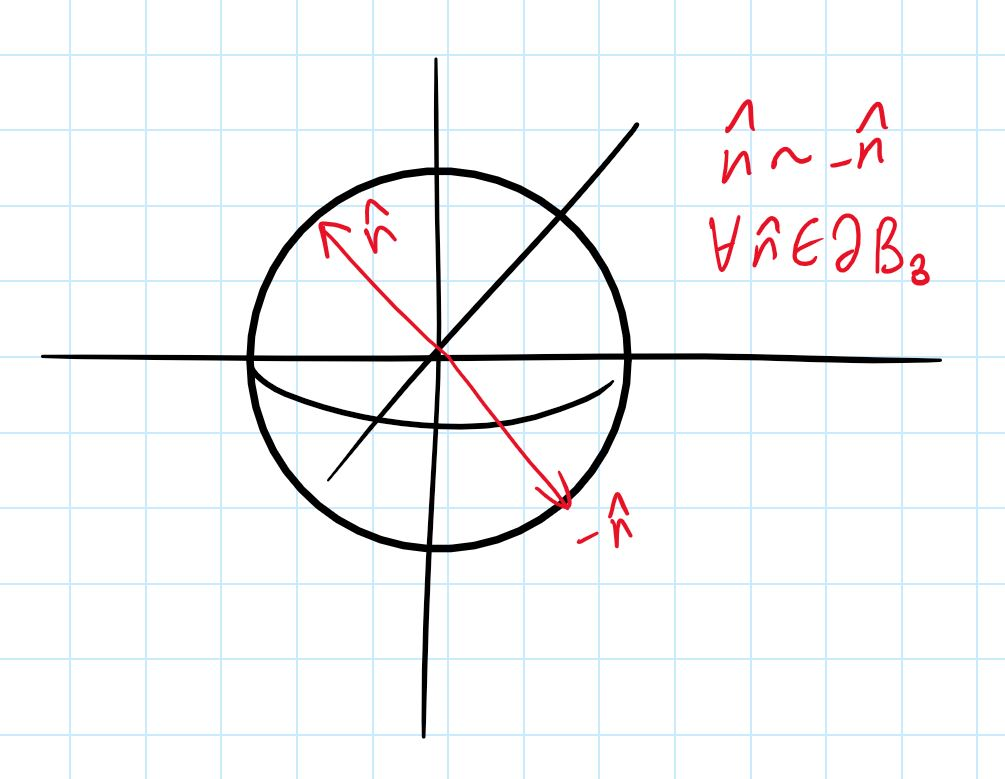
\includegraphics[scale=0.7]{2018/10/20181009_img1}
\caption{The group manifold $M(SO(3))$ is isomorphic to the 3-ball $B^3$ with antipodal points on the boundary identified, $\vec{w} \sim -\vec{w} \forall \vec{w} \in \p B_3$.}
\end{figure}

\begin{defn}
A \term{compact} set is any bounded, closed set in $\RR^n$ with $n\geq 0$.\footnote{This is a sufficient condition but avoids the song and dance about unions of closed sets, etc.} For instance, the $2$-sphere $S^2$ is clearly bounded in $\RR^3$. But the hyperboloid $H^2$ (embedded in $\RR^3$ as $x^2+y^2-z^2 =r^2$) is not bounded, since for any distance $r_0$ one can construct a point $\vec{x}$ on $H^2$ which has $|\vec{x}|>r_0$.
\end{defn}

Let us note some properties of the group manifold $M(SO(3))$. It is compact and connected, but it is not simply connected.
\begin{defn}
A space is \term{simply connected} if all loops on the space are contractible (in the language of algebraic topology, its fundamental group $\pi_0$ is trivial).
\end{defn}
A bit of intuition for why $M(SO(3))$ is topologically non-trivial: draw a path to the boundary, come out on the antipodal side, and go back to the origin. As it turns out, this is different from $S^1$ or the torus $T^2$: whereas these have the full $\ZZ$ as (part of) their fundamental groups ($T^2$ is simply $S^1\times S^1$), if we go around twice in $SO(3)$ we find that this new loop is actually a trivial loop (see Fig. \ref{z2inso3}). Therefore the fundamental group of $SO(3)$ is not infinite but the cyclic group $\ZZ_2$ (i.e. the set $\set{0,1}$ under the group operation $+\mod 2$).

\begin{figure}\label{z2inso3}
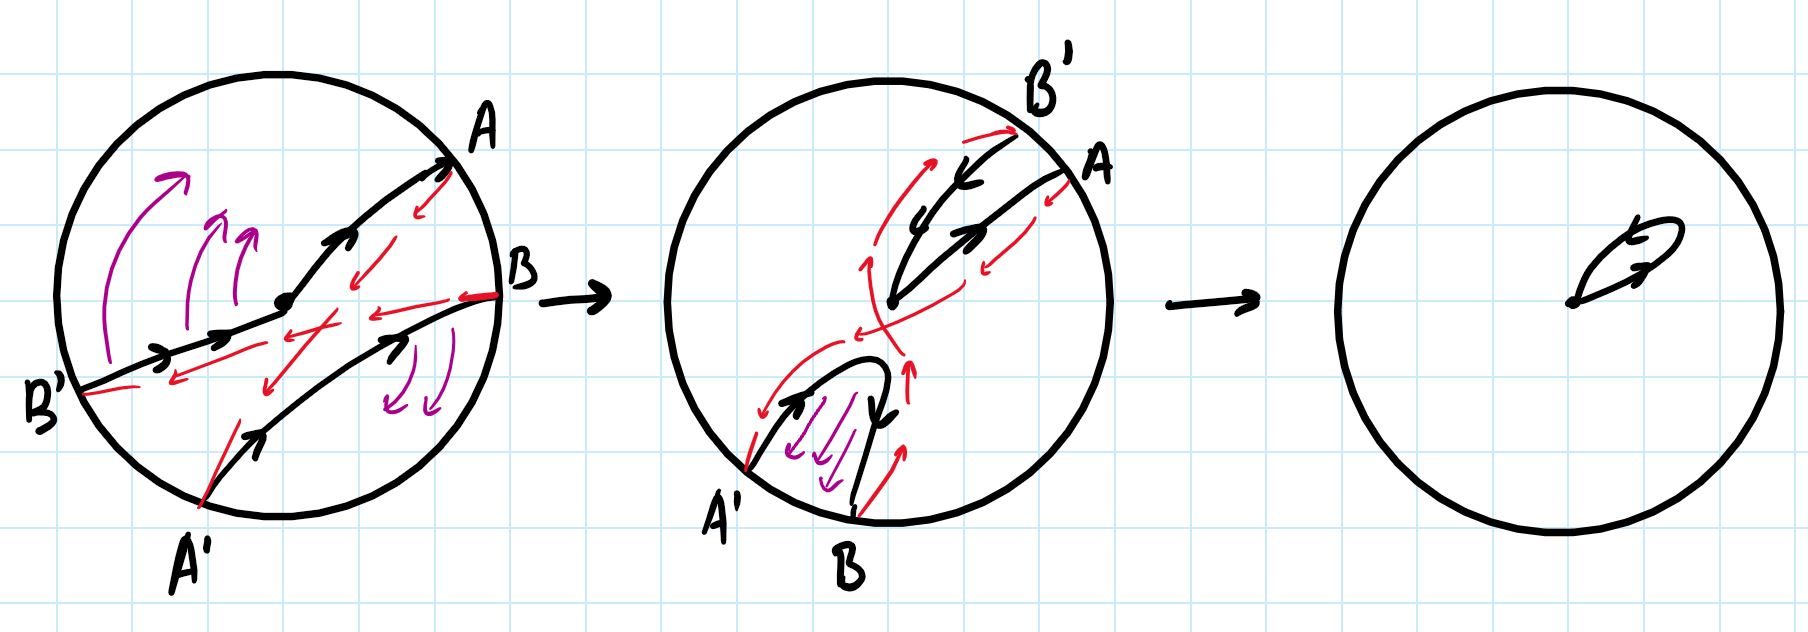
\includegraphics[scale=0.6]{2018/10/20181009_img2}
\caption{A sketch of why the loop which goes through the boundary $\p B_3$ twice is homotopic to (can be continuously deformed into) the trivial loop. For simplicity, consider a circular cross-section of $B_3$ and suppose the loop passes through the boundary at points $A$ ($\sim A'$) and $B$ ($\sim B'$). As we continuously move the point $B$ to $A'$, $B'$ must also move towards $A$, as we see in the second image. We then pull the bit of loop from $A'$ to $B$ through the boundary and find that the resulting loop is trivial (sketch 3). Solid black lines indicate the actual loop path, red dashed arrows indicate the effect of identifying antipodal points, and purple arrows suggest the direction of loop deformation between each drawing.}
\end{figure}